\section{Method}
\label{sec:method}

\begin{figure*}[t]
  \centering
  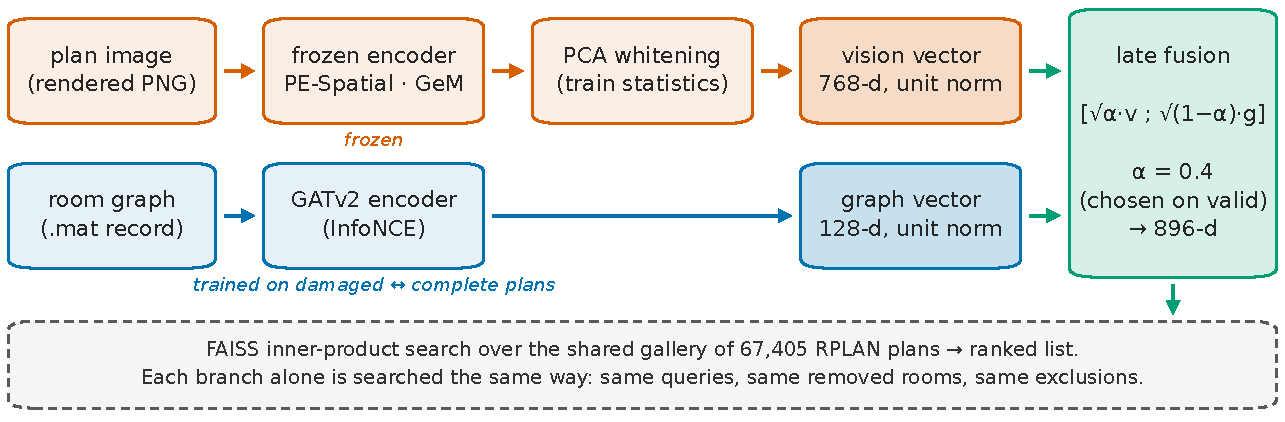
\includegraphics[width=\textwidth]{figures/english/f_final_pipeline_readme.pdf}
  \caption{\textbf{FusePlan pipeline.}
  The vision branch embeds the rendered plan with a frozen encoder and whitening; the graph branch embeds the room graph with a GNN trained to map partial plans onto complete ones.
  Late fusion concatenates the two unit vectors with weights $\sqrt{\alpha}$ and $\sqrt{1-\alpha}$ ($\alpha=0.4$ with the frozen branch, chosen on validation), so one inner product scores both.
  The damage-trained vision variants (\cref{sec:method_vision}) add a trained head to the vision branch and choose their own $\alpha$ with the same rule.
  An exact inner-product FAISS search ranks the gallery of 67{,}405 plans with the fused vector; each branch alone is searched the same way, with the same queries and removed rooms.}
  \label{fig:pipeline}
\end{figure*}

% Sources (paper-comp/CVCS-AI-Assisted-ID/): PAPER.md §5.1, §5.5-§5.8;
% fusion src/evaluation/{query_vectors,late_fusion,fusion_select}.py;
% weights results/csv_final/{valid,test}_seeds.csv (alpha_main 0.4 in 4/4, alpha_head 0.3/0.4),
% results/csv_multiseed/head_v2_fusion.csv (0.6/0.6/0.5/0.5);
% graph configs/graph_models/gat.yaml, results/csv_final/valid_graph_selection.csv (gat/comb, 317952 params);
% vision configs/vision_models/pespatial.yaml, src/vision/models/vision_encoders/base.py:10-12 (clamped GeM).
% alpha rule src/evaluation/fusion_select.py:106-130 (ties, median, closer to 0.5); ties [0.3, 0.4] in
% results/final_pipeline/fusion/s*/select_valid.json; curve grid src/evaluation/fusion_curve.py:43,135-136; heads src/vision/models/projection_head.py
% (single-damage 768->1024->256, configs/vision_retrieval.yaml:30-33; multi-damage residual 768->1024->768);
% graph out_dim 128 in configs/graph_models/*.yaml, no variant of src/graph/final_graph_configs.py changes it.

Let $\mathcal{G}$ be a gallery of floor plans, each available as a rendered image and as a structural record (room types, room boxes, typed adjacencies).
A query $\tilde{q}$ is a plan $q\in\mathcal{G}$ with part of its content removed (\cref{sec:metrics}).
The task asks for a ranking of the whole gallery that places the source plan $q$ as high as possible.
A vision encoder maps a plan to a unit vector $v$ ($v\in\mathbb{R}^{768}$ for the frozen branch, $\mathbb{R}^{256}$ for the single-damage head of \cref{sec:method_vision}) and a graph encoder maps it to a unit vector $g\in\mathbb{R}^{128}$, the size shared by every graph encoder we train.
Both branches index the same gallery and receive the same damaged queries, so we compare branches and fusions query by query (\cref{fig:pipeline}).

\subsection{Late fusion and ensemble controls}
\label{sec:method_fusion}

\paragraph{Fusion.}
The fused descriptor concatenates the two L2-normalised vectors with a single weight $\alpha$; for a query $q$ and a gallery plan $p$,
\begin{equation}
  \begin{gathered}
  z = \bigl[\sqrt{\alpha}\,v \,;\, \sqrt{1-\alpha}\,g\bigr],\\
  \langle z_q, z_p\rangle = \alpha\,\langle v_q, v_p\rangle + (1-\alpha)\,\langle g_q, g_p\rangle,
  \end{gathered}
  \label{eq:fusion}
\end{equation}
where $\langle\cdot,\cdot\rangle$ is the inner product, equal to the cosine similarity for unit vectors.
Hence $\lVert z\rVert=1$, and one exact inner-product FAISS search over the concatenated vectors (896-d with the frozen branch) ranks the gallery by a weighted average of the vision and graph cosine similarities, with weights $\alpha$ and $1-\alpha$.
At $\alpha=1$ and $\alpha=0$ the fusion reproduces the two branches, which we use as a correctness check.
For a damaged query, both branches recompute the query vector from the \emph{same} removed rooms; gallery vectors always describe complete plans.
We choose $\alpha$ on the validation split over $\{0, 0.1, \dots, 1\}$ with a rule fixed before the runs.
The criterion is the robustness to room removal (\cref{sec:metrics}), the only damage both branches can receive.
Neighbouring weights often score almost the same, so the arg-max would pick one of them by chance.
We therefore compare every $\alpha$ with the best one on the same queries: when the 95\% bootstrap interval of their paired difference contains zero (\cref{sec:metrics}), the two count as tied, and we take the median of the tied values (of two central values, the one closer to 0.5).
For $W$ with the frozen vision branch, 0.3 and 0.4 tie in all four replicas and the rule gives $\alpha^*=0.4$; every other fusion selects its own weight with the same rule (the graphs of \cref{fig:curve} on the coarser grid $\{0, 0.2, \dots, 1\}$), and the test split uses the weights fixed on validation.
The fusion is static: every query uses the same $\alpha$, and no gate adapts the weight to the single query, for instance to how much of it is missing.

\paragraph{Ensemble controls.}
Fusing any two models with partly independent errors raises retrieval accuracy, so a fusion gain alone does not show that the image carries information the graph lacks.
We therefore compare every vision--graph fusion with two \emph{ensemble controls} that fuse the graph with a second model holding the \emph{same} information: a second training of the same graph configuration (different initialisation and batches), and a graph encoder of another family trained with the same recipe.
Each control selects its own weight on validation with the rule above.
For a fusion $F$ of branches $A$ and $B$, the per-query gain is $\mathrm{gain}_F(q)=\mathrm{AUC}_F(q)-\mathrm{AUC}_{b}(q)$, where $b$ is the branch with the higher mean AUC.

\paragraph{Complementarity gain.}
We call \emph{complementarity gain} the part of a vision--graph gain that no second graph model provides,
\begin{equation}
  \mathrm{CG} = \overline{\mathrm{gain}}_{V+G} - \overline{\mathrm{gain}}_{C^\star},
  \label{eq:cg}
\end{equation}
where $C^\star$ is the ensemble control with the larger mean gain, a conservative choice.
We compute CG query by query, on the same queries for both fusions, with a 95\% bootstrap interval (\cref{sec:metrics}).
$\mathrm{CG}>0$ means the vision branch contributes information beyond an ensemble effect; the remaining part $\overline{\mathrm{gain}}_{C^\star}$ is what a second graph model would already deliver.
The two parts come from different fusions, so they summarise the gain and do not split one fusion additively.

\subsection{Graph branch}
\label{sec:method_graph}

\paragraph{Room graph.}
We build each graph from the RPLAN record~\cite{wu2019rplan}, not from the image.
Each room becomes a node whose 19 features concatenate a one-hot encoding of the 13 room types with the centre, width, height, area and aspect ratio of the room box on the $256\times256$ RPLAN grid; we clip the aspect ratio at its 99th percentile and standardise the geometric features.
Each adjacency becomes an undirected edge with a one-hot encoding of the 10 RPLAN relation types.

\paragraph{Encoder.}
The encoder $W$ stacks three GATv2 layers~\cite{brody2022gatv2} with hidden size 256, one attention head and edge features in the attention.
We sum-pool the node states and concatenate the sum-pooled input features; on the one-hot part this skip connection equals the room-type histogram.
A linear layer projects the result to 128 dimensions, followed by L2 normalisation (317{,}952 parameters).

\paragraph{Training for incompleteness.}
We train with the symmetric InfoNCE loss~\cite{oord2019cpc}, in-batch negatives, temperature $\tau=0.1$, batch size 256, learning rate $10^{-3}$, weight decay $10^{-5}$ and no dropout, on the training split only.
Positive pairs are \emph{asymmetric}: one view is the complete plan, the other removes a fraction $f\sim\mathcal{U}[0.25,0.75]$ of its rooms together with their edges.
The pair thus asks the encoder to map a partial plan onto its complete version, the retrieval task itself.
We select the checkpoint on retrieval, not on the loss: after each epoch we measure the robustness to room removal on 2{,}000 validation queries disjoint from the evaluation queries, with the whole gallery, over 600 epochs.
The selected epoch falls between 550 and 592 in all four replicas, so the reported robustness of the graph is a lower bound.

\paragraph{Configuration search.}
We chose $W$ with the same recipe for GCN~\cite{kipf2017gcn}, GraphSAGE~\cite{hamilton2017graphsage} and GATv2.
Starting from a reference configuration per encoder, we changed one factor at a time: temperature, skip connection, rotation and reflection augmentation, a lost-neighbour marker, depth, width, pooling, aggregator and attention heads.
We then combined the changes that improved robustness in all four seeds.
We train each of the 37 candidates with 4 seeds and score it on validation only (\cref{tab:ablation_graph}).
$W$ is the combination for GATv2: $\tau=0.1$, no rotations or reflections, three layers, width 256 and one head.

\subsection{Vision branch}
\label{sec:method_vision}

\paragraph{Frozen encoder.}
The vision branch uses the spatially aligned Perception Encoder~\cite{bolya2025perception} (PE-Spatial, ViT-B/16) without training.
We resize the rendered plan so that its longer side has 224 pixels, keeping the aspect ratio, and pad it to a square with the white background.
The descriptor is the generalised mean (GeM~\cite{radenovic2019gem}) with $p=3$ of the last-layer patch tokens $x_1,\dots,x_N$, computed per channel as $\bigl(\tfrac{1}{N}\sum_i \max(x_i,\epsilon)^p\bigr)^{1/p}$ with $\epsilon=10^{-6}$.
The clamp at $\epsilon$ comes from the standard GeM implementation, designed for CNN activations that are non-negative after the ReLU.
ViT tokens after the final LayerNorm are signed, so here the clamp zeroes their negative components and the descriptor pools only the positive part of each channel.

\paragraph{Whitening and indexing.}
We apply PCA whitening~\cite{jegou2012whitening}: mean and covariance come from training-split plans only, and every descriptor $x$ maps to $\Lambda^{-1/2}U^\top(x-\mu)$, keeping all 768 components, followed by L2 normalisation.
An exact inner-product FAISS index~\cite{douze2025faiss} stores the gallery.
Whitening matters because the frozen descriptors of the synthetic renderings collapse into a narrow cone; it improves robustness in all 26 encoder, pooling and resolution settings we tested (\cref{tab:ablation_vision}).
PE-Spatial with this pooling and whitening is the most robust of 52 frozen configurations over 8 encoders~\cite{oquab2024dinov2,simeoni2025dinov3,tschannen2025siglip2,ranzinger2024amradio,assran2023ijepa,cao2026tipsv2,bolya2025perception}, selected on validation.

\paragraph{Damage-trained heads.}
To test whether a vision branch trained on the damage carries more information, we train two alternative heads on top of the frozen encoder; each one replaces the frozen branch in its own fusion, and the two are never stacked.
Both train with InfoNCE ($\tau=0.07$, batch 4{,}096) on training plans, with self-supervised positives and no relevance labels.
The \emph{single-damage head} is an MLP ($768\to1024\to256$, GELU) applied to gallery and queries; it learns to match a plan with rooms removed to the complete plan, and we re-estimate the whitening on its 256-d outputs.
The \emph{multi-damage head} acts on queries only: it adds a residual MLP ($768\to1024\to768$, last layer initialised at zero) to the whitened frozen vector, so the gallery stays frozen; it trains on room removal, crop and patch in turn.
Both heads select their epoch on 1{,}000 validation queries disjoint from the evaluation queries.
